\chapter{Power Grid Reliability Estimation via Adaptive Importance Sampling}
\label{chap:sampling}
This chapter is based on the publication of the dissertation author: \fullcite{lukashevich2021power}
\section{Introduction}
\label{sampling:introduction}

Carbon-free electricity generation is one of the most vital global challenges for the next decades. Because of their ecological and economic benefits, renewable energy sources, such as wind, hydro, and solar power generation, become more demanded, accessible, and widely used in modern power grids \cite{harjanne2019abandoning}. For instance, California's renewable portfolio standard currently requires 33\% of retail electricity sales to come from renewable resources, and will require 60\% by 2030, and 100\% by~2045~\cite{golden2003senate}.
However, renewable energy generation is highly volatile and brings significant uncertainty to power systems. This also gives rise to many challenges for power system operators trying to integrate renewables into power grids \cite{schmietendorf2017impact}. In particular, power systems operational policies and reliability assessment must be verified over various additional uncertainties, including increased variation in power generation and disturbances. 

Various algorithms have been developed so far for ensuring grid reliability. Some of them are based on machine learning, and utilize historical data about weather, renewables' generation, and grid operating parameters to estimate the risk of overload and influence of uncertainty due to weather changes~\cite{zhang2017data}. %,contingencyMLE}.
%3contingencymethods,
%,zhou2019wind
Requiring large datasets and high data collecting time to make an accurate prediction, machine learning methods become impractical for real-time operation if a large disturbance, contingency, or a sudden operational policy change precedes the reliability assessment. Another class of algorithms is based on analytical approximation of the overload probability~\cite{nemirovski2007convex}. In this approach, the risk of interest is upper-bounded by an integral of an appropriate function that admits analytical or numerical computation. However, even in the simplest case of linear reliability constraints and Gaussian fluctuations of renewables, existing approaches tend to overestimate the risk. Moreover, for a sufficiently rare event, the risk overestimation for these algorithms can be infinitely high~\cite{nemirovski2007convex} which compromises their practical~efficiency. 

Finally, algorithms based on sampling values of power generated by renewables and approximating the grid constraints overflow probability by its empirical counterpart often provide a valuable alternative for accessing the reliability posture of a power system. Monte-Carlo (MC), hybrid and Markov Chain MC have been earlier applied to risk-based reliability assessment of transmission power grids~\cite{su2005probabilistic,vittal2009steady,chen2008probabilistic}. 
%da1990probabilistic,
In~\cite{montecarlofeasibility}, the authors exploited Monte Carlo simulation for estimating overload probability and interpreted the risk by classifying it into low, medium and high risk operating points. Variations of the load-flow solution due to renewables fluctuation, nodal and line parameters uncertainty were considered in~\cite{su2005probabilistic}.  An inverse problem of wind turbine controls to meet reliability margins with high-probability is discussed in \cite{vittal2009steady}.  A comprehensive survey of sampling-based methods for power systems reliability assessment is given in~\cite{chen2008probabilistic}.
Unfortunately, these algorithms explore the space of fluctuations uniformly, which dramatically 
reduces their performance in understanding and evaluating the effect of a rare event such as a severe disturbance. 

Importance sampling is a valuable alternative to Monte-Carlo sampling, which allows adjusting distribution for generating more samples in the areas of interest, e.g., close to the reliability boundary. Pmvnorm~\cite{genz2020package} is one of the most efficient importance sampling algorithms in general, but its performance is often limited for rare events probability estimation~\cite{owen2019importance}, which is of the utmost importance to power systems study.  ALOE~\cite{owen2019importance}~is another efficient method designed especially for computing a rare event probability. However, it does not fully respect the geometry of reliability constraints. 
It thus requires a large number of samples to estimate the risk of constraint overflow, especially for large power grids and multi-line overloads. Finally, a convex optimization-based algorithm for adaptive importance sampling from exponential families was proposed in~\cite{ryu2014adaptive}. At each step, the algorithm adjusts the distribution parameters so that the sampler's variance is minimized. Unfortunately, the distribution of output power that leads to an overload is far from the exponential family,  limiting the algorithm's efficiency in power systems.

This chapter proposes an adaptive importance sampling method to efficiently estimate the risk of reliability constraints violation.
We present an importance sampling algorithm that uses physical information to generate a mixture of distributions to sample from and then uses convex optimization to iteratively adjust the weights of the mixture. Our algorithm substantially improves static weights assignment of ALOE~\cite{owen2019importance} when reliability constraints are highly correlated.
The approach allows to address the risk estimation problem in real-time even for large power grids with a small constraint overflow probability. We theoretically analyze the accuracy and complexity of our algorithm for the case of Gaussian power fluctuations from renewables; however, the technique is not limited to the Gaussian case. Finally, we evaluate the performance of our sampling methods over multiple real and synthetic test cases and compare it to the state-of-the-art. 

The chapter is organized as follows. 
In Section \ref{sampling:setup} we present the constraint overload probability estimation problem and introduce notation used in the chapter. We outline the importance sampling algorithm and present its theoretical analysis in Section \ref{sampling:prob}. Empirical study and comparison to the state-of-the-art are given in Section~\ref{sampling:emp}. In Section~\ref{sampling:conclusion} we conclude  with a brief summary and possible applications of our results. 

\section{Background and Problem Setup}\label{sampling:setup}

Being a popular load flow model, the higher-voltage direct current (DC) model remains simple for the analysis because of linear relations between power injections and phase angles. Let $G = (V, E)$ be a power grid graph with a set of buses~$V$, $|V| = n$ and a set of lines~$E$, $|E| = m$. Let $p \in \mathbb{R}^{n}$ and $\theta\in\mathbb{R}^{n}$ be vectors of power injections and phase angles respectively.  The power system is balanced, e.g., the sum of all power injections equals zero $\sum_{i \in V} p_i = 0$. To avoid ambiguity let $s$ be the slack bus and $\theta_s = 0.$ Let $B \in \mathbb{R}^{n \times n}$ be an admittance matrix of the system, $p = B\theta$. The components $B_{ij}$ are such that $B_{ij} \neq 0$ if there is a line between buses $i$ and $j$ and  for any node $B_{ii} = - \sum_{j\neq i} B_{ij}$, e.g., $B$ is a Laplacian matrix.  Let $B^{\dagger}$ be the pseudo-inverse of $B$, $\theta = B^{\dagger} p$. The DC power flow equations, generation and reliability constraints are 
\begin{subequations}
\label{eq:DC-PF}
    \begin{equation}
        p = B \theta
        \label{eq:DC-PF-a}
    \end{equation}
    \begin{equation}
        \underline{p}_i \leq p_i \leq \overline{p}_i
        \label{eq:DC-PF-b}, i \in V \text{ and } |\theta_i - \theta_j| \leq \bar{\theta}_{ij}, \; (i,j)\in E
    \end{equation}
    %\begin{equation}
    %    |\theta_i - \theta_j| \leq \bar{\theta}_{ij}, \; (i,j)\in E
    %    \label{eq:DC-PF-c}
    %\end{equation}
\end{subequations}
Reliability constraints~\eqref{eq:DC-PF-b} %, \eqref{eq:DC-PF-c} 
define a polytope $P$ in the space of power injections, $P = \{p: W p \le b\}$, so that the reliability constraints are violated if and only if power injections $p \not\in P.$ 

To derive an explicit expression of matrix $W$ we consider the incidence matrix $A$, such that for any buses $i$ and $j$ with $i<j$ connected by an edge $k$, $A_{ki} = 1$, $A_{kj} = -1$ and all other elements in row $k$ are equal to zero. Then the phase angle constraints are $AB^{\dagger}p \le \bar\theta$, $-AB^{\dagger}p \le \bar\theta$. 
%
Finally, as the slack bus balances the system, $p_s = -\sum_{i\neq s} p_i$ let $C \in \mathbb{R}^{n\times n}$ be a symmetric matrix such that for any non-slack buses $i$ and $j$, and the slack bus $s$, $C_{ii} = 1$, $C_{ij} = 0$, $C_{ss}=0$, and $C_{is} = -1$. In other words, $C p$ is a vector of grid power injections expressed in terms of non-slack injections only, since the slack bus power injection is fully determined by the other ones. 


Finally, from Eqs.~\eqref{eq:DC-PF} the following system of inequalities defines the reliability polytope, $P = \{p: Wp \le b\}$,
\begin{equation}
(AB^\dagger C, - A B^\dagger C, C, -C)^\top p \le (\bar\theta, \bar\theta, \overline{p}, \underline{p})^\top, 
\label{eq:feasibility_ineqs}
\end{equation}
with $W = (AB^\dagger C, - A B^\dagger C, C, -C)^\top$, $b = (\bar\theta, \bar\theta, \overline{p}, \underline{p})^\top$\!\!\!. Let $K = 2m + 2n$ be a number of constraints, e.g., rows in matrix $W$, then the reliability polytope $P$ is $\bigl\{p\!:\! \bigcap_{i=1}^K p^\top\!\!\omega_i \le b_i\bigr\}$. 

Stochastic uncertainty in renewable generation and power consumption imposes a question of power grid reliability, e.g., estimating a probability that at least one of the reliability constraints is violated. Namely, we consider Gaussian fluctuations of power injections $p$ with known mean $\mu$ and covariance $\Sigma$ and aim at computing a constraint violation probability $\Pi$:
\begin{align}\label{eq:prob}
    \Pi = \mathbb{P}(p\not\in P) = \int_{\mathbb{R}^n} \upsilon(p) 1[p\not\in P] d p, \; p\sim \mathcal{N}(\mu, \Sigma), 
\end{align}
where $\mathbb{P}$ is a probability taken w.r.t. the normal pdf $\upsilon(p)$ of $p$. 

Notice, that the probability $\Pi$ does not have an analytic expression, it is computationally intractable, and even hard to approximate~\cite{owen2019importance,ryu2014adaptive,cappe2008adaptive, khachiyan1989problem}. 
In practice, a union bound is often used to upper bound $\Pi$. Let $\Pi_i$ be a probability of a single event, e.g., $p^\top\omega_i > b_i$. It has an explicit expression for the Gaussian distribution, and by union bound inequality
$\sum_{i\le K}\Pi_i \ge \Pi \ge \max_{i\le K} \Pi_i$. However, the bounds are loose when dealing with correlated violations which is often the case for power systems. 

To refine the overload estimate and take into account simultaneous violation of multiple constraints, we propose an importance sampling procedure that allows to count the average number of constraints $N$ violated at the same time and, thus, improve the overload probability estimation to $\Pi/N$ instead of $\Pi$. It is meaningful for large power grids where multiple events are likely to happen synchronously.

Table~\ref{tab:notation_sampling} summarizes chapter's notation. We use lower indices for elements of vectors and matrices, lower-case letters for probability density functions (pdfs), and upper-case letters for cumulative distribution functions (cdfs). When it does not lead to confusion, we use $\mathbb{P}$, $\mathbb{E}$, $\mathbb{V}$ to denote  probability, expectation, and variance without explicitly mentioning a distribution. 

\begin{table}[t]
    \centering
    \caption{Chapter notation.}
    \begin{tabularx}{\textwidth}{|m{1cm}|X|m{1.5cm}|X|}
        \toprule
        $E$ & set of lines, $|E| = m$ & $\upsilon(p)$ & nominal distribution pdf\\
        $V$ & set of buses, $|V| = n$ & $\upsilon_D$ & parametric distribution pdf\\
        $B$ & $n\times n$ admittance matrix& $x$ & mixture distribution para- \\
        $p_i$ & power injection & & meters, $x\in X \subseteq \mathbb{R}^K$\\
        $\underline{p}_i$ & lower generation limit & 
        $D_i$& $p\!\sim\!\mathcal{N}(\!\mu, \!\Sigma)$ s.t. $p^\top\! \omega_i \!> \!b_i$\hspace{-5mm}\\
        $\overline{p}_i$ & upper generation limit & $N$ & number of samples\\
        $\theta_i$ & phase angle & $\mathbb{P}$, $\mathbb{E}$ & probability, expectation\\
        $\theta_{ij}$ & phase angle difference%, $\theta_i - \theta_j$
        &$\mathbb{V}$, $\kl$ & Variance, KL-divergence\\
        $\bar\theta_{ij}$ & angle difference limits & ${\mathcal{N}}\!(\mu, \!\Sigma)\hspace{-5mm}$ &  Gaussian distribution with\\
        $I_n$ & $n\times n$ identity matrix & & mean $\mu$ and covariance $\Sigma$\\
        $K$ & number of constraints & $\Phi$ & ${\mathcal{N}}(0,1)$ distribution cdf\\ 
        ${P}$ & reliability set, $p\!:\! W p \!\le\! b\!\!\!\!$ & $U(0,1)$ & uniform $(0,1)$ distribution\\
        $\omega_i$ & rows of matrix $W$, $i\le K$ & $\Pi$ & overflow probability, $\!p\not\in\! P$ \\
        \bottomrule
    \end{tabularx}
    \label{tab:notation_sampling}
    % \vspace{-4mm}
\end{table}


\section{Overload Probability Estimation}\label{sampling:prob}

\subsection{A Single Constraint Case}
We start with estimating the probability of fluctuating power injections to cause an overload of an individual constraint, e.g., $\Pi_i = \mathbb{P}(p^\top \omega_i \ge b_i)$ for some $i$, $1\le i \le K$. In the case of a Gaussian distribution, $p\sim \mathcal{N}(\mu,\Sigma)$ there is a closed form expression for it:
% \begin{align*}
% \Pi_i & = \mathbb{P}_{p\sim \mathcal{N}(\mu, \Sigma)}(p^\top \omega_i \ge b_i)  = \mathbb{P}((p - \mu)^\top \omega_i \ge b_i - \mu^\top \omega_i)\\
% & = \mathbb{P}_{{\tilde p}\sim \mathcal{N}(0, I_n)} \left((\Sigma^{1/2}\omega_i)^\top {\tilde p} \ge b_i - \mu^\top \omega_i\right) \\
% & = \mathbb{P}_{{\tilde p}\sim \mathcal{N}(0, I_n)} \left( {\tilde p}^\top {\bar\omega}_i \ge (b_i - \mu^\top \omega_i)/\|\Sigma^{1/2}\omega_i\|_2\right)  \\
% & = \Phi((b_i - \mu^\top \omega_i)/\|\Sigma^{1/2}\omega_i\|_2), 
% \end{align*}
$%$\begin{align*}
\Pi_i  = \mathbb{P}_{p\sim \mathcal{N}(\mu, \Sigma)}(p^\top \omega_i \ge b_i) %\\
%& = \mathbb{P}_{{\tilde p}\sim \mathcal{N}(0, I_n)} \left( {\tilde p}^\top {\bar\omega}_i \ge (b_i - \mu^\top \omega_i)/\|\Sigma^{1/2}\omega_i\|_2\right)  \\
 = \Phi((b_i - \mu^\top \omega_i)/\|\Sigma^{1/2}\omega_i\|_2), 
$%\end{align*}
where $\Phi$ is the standard Gaussian distribution cdf, ${\tilde p} = \Sigma^{-1/2}(p-\mu)$, ${\bar\omega}_i = (\Sigma^{1/2}\omega_i)^\top/\|\Sigma^{1/2}\omega_i\|_2$, and $1\le i \le K$. $\Pi_i$ are the probabilities of $p^\top \omega_i \ge b_i$, so that 
$
    \Pi = \mathbb{P}(\exists i: p^\top \omega_i \ge b_i) \le \sum_{i\le K}\mathbb{P}(p^\top \omega_i \ge b_i) = \sum_{i\le K} \Pi_i.
$

Algorithm~\ref{alg:sample1d} is an instance of the inverse transorm method \cite{l2009monte} which allows to sample $p \sim \mathcal{N}(\mu, \Sigma)$ s.t. $p^\top \omega_i > b_i$. We refer this distribution as $D_i$, and its pdf is $\upsilon(p)/\Pi_i$ if $p^\top \omega_i > b_i$ and $0$ otherwise. Notice, that sample $p \sim \mathcal{N}(\mu, \Sigma)$ can be obtained with the plain MC from $\mathcal{N}(\mu, \Sigma)$, but it requires on average $1/\Pi_i$ trials instead of just one for Algorithm~\ref{alg:sample1d}.

\begin{algorithm}[H]
    \SetKwInOut{Input}{input}
    \SetKwInOut{Output}{output}
    \caption{Sampling $p\sim \mathcal{N}(\mu,\Sigma)$ s.t. $p^\top \omega_i \geq b_i$}
    \label{alg:sample1d}
    \Input{Mean $\mu$, covariance $\Sigma$, and a constraint $p^\top \omega_i \le b_i$} 
    \Output{$p\sim\mathcal{N}(\mu,\Sigma)$ s.t. $p^\top \omega_i \ge b_i$}
    Sample $z \sim \mathcal{N}(0, I_n)$ and $u \sim U(0,1)$\;
    Compute $y = \Phi^{-1}(\Phi(\tau) + u(1 - \Phi(\tau)))$\;
    Set $\phi = \bar\phi y + (I_n - \bar\phi\phi^\top) z$, with $\bar\phi = \Sigma^{1/2} \omega_i / \|\Sigma^{1/2} \omega_i\|_2$\!\! \;
    \Return $p = \Sigma^{1/2} (\phi+\mu)$
\end{algorithm}

 
 \subsection{Multiple Constraints Case}
 
The case of multiple constraints is more involved. Indeed, there is no analytical formula for an overload probability and, moreover, its exact computation is intractable~\cite{khachiyan1989problem}. 
%The plain 
Monte-Carlo sampling, $p\sim \mathcal{N}(\mu, \Sigma)$ is inefficient in estimating the constraint overload probability, especially if it is small. Indeed, it requires on average $O(1/\Pi)$ samples to get at least one of the outside the reliability polytope, $p\not\in P$. 

The importance sampling idea is to change the distribution one samples from and assign a weight to each sample to account for the~change: 
\begin{align*}
    \Pi  = \mathbb{P}(p\not\in P) & = \int_{\mathbb{R}^n} f(p) \upsilon(p) dp = \!\int_{\mathbb{R}^n}\!\! \frac{f(p)\upsilon(p)}{\upsilon_D(p,x)}\upsilon_D(p,x) dp%\\
    %& \approx \frac{1}{N}\sum_{i=1}^N \frac{f(p^i)\upsilon(p^i)}{\upsilon_D(p^i,x)}, p^i \sim %\upsilon_D(p,x),
\end{align*}
where we refer to $\upsilon(p)$ as \emph{nominal} distribution, and $\upsilon_D(p,x)$ as \emph{synthetic} distribution with parameter $x$,  $f(p) = 1[p\not\in P]$. 

A natural extension of importance sampling with a single linear constraint to the case of multiple linear constraints is to sample from a mixture distribution: 
%\begin{align}\label{eq:mix}
    $D = \sum_{i \le K} x_i D_i, \text{ with } \sum_{i\le K} x_i = 1, x_i \ge 0, \; 1\le i \le K,$
%\end{align}
where $D_i$ is $\mathcal{N}(\mu,\Sigma)$ conditioned on $p^\top\omega_i > \!b_i$. 
%
The sampling algorithm consists of two steps. First, we choose a distribution $D_i$ with probability $x_i$. Second, we sample $p \sim D_i$, i.e. $p\sim \mathcal{N}(\mu,\Sigma)$ given $p^\top\omega_i>b_i$, according to Algorithm~\ref{alg:sample1d}.
%
Probability density function $\upsilon_D(p, x)$ of $D$ is given by
    $\upsilon_D(p, x) = \sum\limits_{i\le K} x_i \upsilon_i(p) 1[p^\top \omega_i > b_i]/\Pi_i$,
    %
    %\begin{cases}
    %0, & \!\!p \in P,\\
    %\sum_{i\le K} x_i \upsilon_i(p) 1[p^\top \omega_i > b_i], & \!\!p\not\in P,
    %\end{cases}
%\end{align*}
where $1[\cdot]$ is a binary indicator, and 
$%\begin{align*}
    \upsilon_i(p) = \upsilon(p) 1[p^\top\omega_i > b_i]/\Phi((b_i - \mu^\top\omega_i)/\|\Sigma^{1/2}\omega_i\|_2).
$%\end{align*}

In contrast to the classical Monte-Carlo, which explores the uncertainty space uniformly according to the nominal distribution, importance sampling from parametric distribution $\upsilon_D(p,x)$ yields samples only from the area of interest, i.e., $p\not\in P$. 
More specifically, Monte-Carlo generates many samples from the true distribution of power injections to estimate overflow probability, while the proposed approach only samples power injections that lead to an overload and adjusts their weights.
Figure \ref{fig:00} illustrates the difference. The white area stands for generations that do not exceed operating limits. A set of generations leading to at least one constraint violation is in grey. Two or more reliability constraints are not satisfied in the dark grey area. The samples from a nominal distribution and the constructed mixture are marked in red and green respectively.

\begin{figure}
    \centering
    % \vspace{-3mm}
    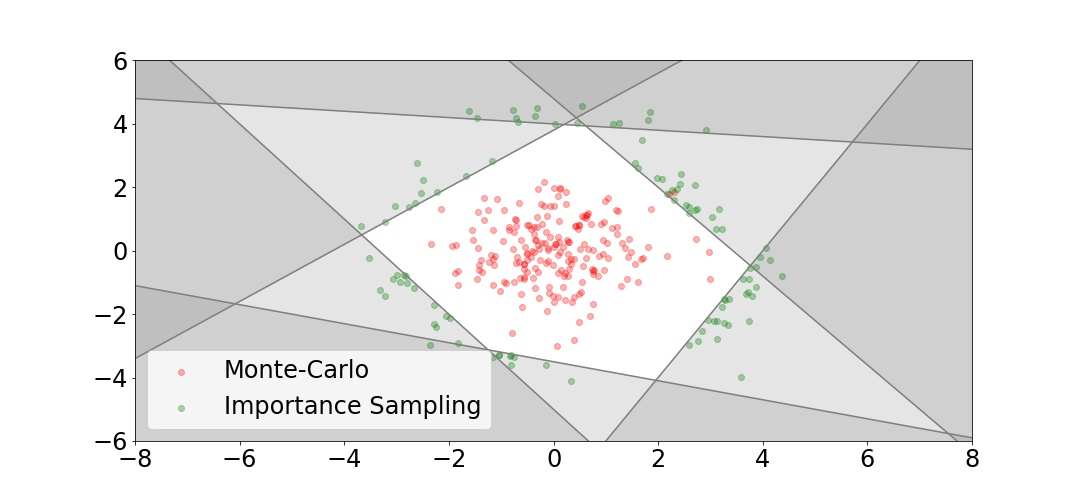
\includegraphics[width=.95\textwidth]{Dissertation/images/sampling/conditioned_vs_MC.jpg}
    % \vspace{-5mm}
    \caption{Samples produced using classical Monte-Carlo approach and using Importance Sampling procedure.}
    \label{fig:00}
    % \vspace{-5mm}
\end{figure}

Having a distribution mixture $\{D_i\}_{i=1}^K$we are looking for the weights $\{x_i\}_{i=1}^K$ to approximate a distribution $D$, $p \sim \mathcal{N}(\mu, \Sigma)$ s.t. $p\not\in P$, in the optimal way. Note that, any positive $\{x_i\}_{i=1}^K$ weights lead to an unbiased estimate 
\begin{align}\label{eq:aloe}
    {\hat \Pi} = N^{-1}\sum_{i=1}^N \upsilon(p^i)/\upsilon_D(p^i, x^i), \quad p^i \sim D^{x^i}
\end{align}
of the probability $\Pi$. Here $x^i$ is the vector of mixture weights for $i^{\textup{th}}$ sample. Indeed, by linearity of the  expectation $\mathbb{E}_{\upsilon_D(p,x)} \hat \Pi = \frac{1}{n}\sum_{i\le n} \int \frac{\upsilon(p^i)1[p^i\not\in P]}{\upsilon_D^{-1}(p^i, x)}\upsilon_D(p^i, x) dp = \Pi$. 

Despite being unbiased for any $x$ with positive components, variance of the  estimate~\eqref{eq:aloe} highly depends on the choice of $x$.
In \cite{owen2019importance} the authors suggested to take $x_i \propto \Pi_i$. 
While it leads to a consistent estimate, the estimator's variance is still high, especially when violation of multiple constraints is likely to happen in the system \cite{owen2019importance}. In practice, it leads to high sample complexity of the estimator which compromises its real time application. In the next subsection, we significantly improve the sampler's efficiency by using convex optimization to find the optimal combination of the mixture distribution weights $x$. 

\subsection{Convexity of Importance Sampling Variance}

We will measure the effectiveness of our estimator by its mean squared error, which is equal to the variance since the estimator is unbiased.
The importance sampler variance is 
\begin{align*}
    \bV_{\upsilon_D(p, x)}\left(\frac{\upsilon(p) f(p)}{\upsilon_D(p, x)}\right) %\int_{p\in\mathbb{R}^n}\!\! \left(\frac{f(p)\upsilon(p)}{\upsilon_D(p, x)} - \Pi\right)^2 %\!\!\upsilon_D(p, x) d p \\
     = \int_{p\in\mathbb{R}^n}\!\! \frac{f^2(p)\upsilon^2(p)}{\upsilon_D(p, x)} d p - \Pi^2 =: V(x), 
\end{align*}
where $f(p) = 1[p\not\in P]$. 

The optimal synthetic distribution can be chosen to minimize the variance, $\upsilon_*(p) = f(p)\upsilon(p)/\Pi$, and thus provide a better approximation to the integral. Notice, that for $\upsilon_D = \upsilon_*$ the variance $V(x) = 0$ and attains its minimum.  However, if $\upsilon_*(p)$ does not belong to the parametric family $\{\upsilon_D(p,x)\}_x$, we are looking for the best approximation of $\upsilon_*(p)$ within it, i.e. a minimum possible value of $V(x)$. 

Figure~\ref{fig:fscheme} illustrates our approach. First, we initialize distributions $D_i$ based on a given set of constraints. Second, we initialize the weights of a mixture distribution to sample  $x_i\propto \Pi_i$. Then, with each new sample from $\sum_{i\le K} x_i D_i$ we update the weight vector $x$ and a overload estimate $\Pi_n$. See Eq.~\eqref{eq:md-upd} for details. In other words, starting from an initial weight assignment, $x_i^1 \propto \Pi_i$, at each iteration $N$ of the algorithm we sample $p^k \sim \upsilon_D(\cdot, x^k)$ and compute $x^{k+1}$ to minimize the variance of the estimate. We also update an empirical estimate of the probability 
\begin{align}
    \hat \Pi = \frac{1}{k}\sum_{t=1}^k \frac{\upsilon(p^t) f(p^t)}{\upsilon_D(p^t, x^t)}, \; p^t \sim \upsilon_D(\cdot, x^t), t\le k \label{eq:emp}
\end{align}
and update parameters $x$ based on the value of $V(x^N)$ and its gradient. Before discussing the update strategy for the parameters $x$, we outline some important properties of the variance $V(x)$ and empirical estimate~\eqref{eq:emp}. 

\begin{figure}
    \centering
    \begin{tikzpicture}[scale=0.7, node distance={15mm}, thick, main/.style = {draw, scale=.9}] 
    \node[main] (a)  {Define distributions $D_i$, \par $p\sim \mathcal{N}(\mu, \Sigma)$ s.t. $p^\top \omega_i\ge b^i$}; 
    \node[main] (b) [below = 4 mm of a] {Choose weights $x$ of the mixture, $p\sim\sum_{i\le K}x_i D_i$}; 
    \node[main] (c) [below = 2 mm of b] {Sample $p \sim \Psi(p, x) = \sum_{i\le K }x_i D_i$}; 
    \node (x) [below = 3 mm of c]{};
    \node[main] (d) [left =  6 mm of x] {Update weights vector $x$};
    \node[main] (e) [right = 4 mm of x] {Update overload estimate $\Pi^N$}; 
    \draw[->] (a) -- (b) node[midway, right] { {\footnotesize set $x_i\propto \Pi_i$}};
    \draw[->] (b) -- (c);
    \draw[<-] (-4.0,-2.3) -- (-4.0,-2.65);
    %\draw[-] (-4.0,-4.9) -- (-4.0,-1.5);
    \draw[->] (c) -- (d); 
    \draw[->] (c) -- (e);
    %\draw[->] (d) -- (e);
    \end{tikzpicture} 
    \caption{Scheme of the proposed estimation algorithm.}
    \label{fig:fscheme}
    % \vspace{-4mm}
\end{figure}

Theorem~\ref{thm:var-convexity} implies convexity of the variance minimization %problem 
\begin{align}
    \min_x \; & V(x), \; 
    \text{s.t. } x_1 + \dots + x_K = 1, x_k \ge 0, 1\!\le\! k \!\le\! K\label{eq:var-min}
\end{align}
in $x$ for the mixture distribution $\upsilon_D(p,x) = \sum_{i=1}^K x_i \upsilon_i(p)$. %To improve numerical stability one may also add constraints $x_i \ge \varepsilon > 0$ that guarantee that the variance is bounded.

\begin{theorem}\label{thm:var-convexity}
Problem~\eqref{eq:var-min} is convex in $x$, and for $x > 0$
\begin{align*}
    \nabla V(x) = \int_{\mathbb{R}^n} - f^2 (p)\upsilon^2(p)\upsilon_D^{-2}(p,x) (\upsilon_1(p), \dots, \upsilon_K(p))^\top dp.
\end{align*} 
\end{theorem}
\begin{proof}
The sub-integral expression, $f^2(p)\upsilon^2(p)/\upsilon_D(p,x)$, is convex for any $x > 0$ as
\begin{align*}
    \nabla^2_x \left[f^2(p)\upsilon^2(p)/\upsilon_D(p,x)\right] = 2f^2(p)\upsilon^2(p)/\upsilon^3_D(p,x) h h^\top \!\succeq\! 0,
\end{align*}
where $h = (\upsilon_1(p), \dots, \upsilon_K(p))^\top = \nabla_x \upsilon_D(p,x)$. 
The latter implies the integral's convexity. %Indeed, the Hessian of the sub-integral expression is non-negative for any $x$ 
Finally, by the dominated convergence theorem as $\mathbb{E}_{p \sim \upsilon_D(\cdot,x)} \nabla_x\left[f^2(p)\upsilon^2(p)/\upsilon_D(p,x)\right]$ is finite for $x>0$, one can exchange the order of differentiation and integration and 
%\begin{align*}
$\nabla V(x) = -\int \frac{f^2 (p)\upsilon^2(p)}{\upsilon_D^2(p,x)} h^\top dp.$
 %\int_{\mathbb{R^n}}\nabla_x \frac{f^2(p)\upsilon^2(p)}{\upsilon_D(p,x)} dp 
 %
%\mathbb{E}_{p \sim \upsilon_D(\cdot,x)} & 
%\left[- \frac{f^2(p)\upsilon^2(p)}{\upsilon_D^2(p,x)}h^\top\right] = \
%\mathbb{E}_{p \sim \upsilon_D(\cdot,x)} % z\nabla_x\!\!\left[\frac{f^2(p)\upsilon^2(p)}{\upsilon_D(p,x)}\right] \\
%& = 
%    \nabla_x \mathbb{E}_{p \sim \upsilon_D(\cdot,x)}  %\left[\frac{f^2(p)\upsilon^2(p)}{\upsilon_D(p,x)}\right] = \nabla V(x).%,
%\end{align*}
%which concludes the proof of the theorem. 
\end{proof}


\begin{theorem}\label{thm:unbias}
$\hat \Pi$ is an unbiased estimate of $\Pi$ if for all $k$, $1\le k \le N$, $x_k > 0$ and $x_k$ is independent of $x^j$ and $p^j$ for~$N\ge j > k\ge 1$.
\end{theorem}
\begin{proof} 
By the law of total expectation for $f(p) \!=\! 1[p\!\not\in\! P]$
\begin{align*}
    \mathbb{E}\, {\hat\Pi} & = \frac{1}{N}\sum_{k=1}^N  \mathbb{E}\biggl[\mathbb{E}_{p^k\sim\upsilon_D(p, x^k)} \biggl[ \frac{\upsilon(p^k) f(p^k)}{\upsilon_D(p^k,x^k)}\big| x^k\biggr]\biggr] = \Pi, %\sum_{i=1}^n \frac{\Pi}{n}= \Pi,
\end{align*}
as $\mathbb{E}_{p^k} \bigl[ \frac{\upsilon(p^k)f(p^k)}{\upsilon_D(p^k,x^k)}\big| x^k\bigr] = \Pi$. %\!=\! \int \frac{\upsilon(p^k)1[p^k \not\in P]}{\upsilon_D(p^k,x^k)}\upsilon_D(p^k,x^k) dp^k
\end{proof}

According to Theorem~\ref{thm:unbias}, the importance sampling estimate is unbiased. Theorem \ref{thm:var} bounds the variance of $\hat\Pi$. 

\begin{theorem}\label{thm:var}
Variance of $\hat\Pi$ equals $N^{-2}\sum_{k=1}^N V(x^k)$ if for all $k$ and $j,$ $1\le k < j \le N$, $x_k > 0$ and $x_k$ is independent of $x^j$ and~$p^j$.
\end{theorem}
\begin{proof} For $f(p) = 1[p\not\in P]$, $\mathbb{V} (\hat\Pi)\!=\! \mathbb{E}(\hat\Pi - \Pi)^2$ one has 
\begin{align*}
    &\mathbb{V}(\hat\Pi) = \frac{1}{N^2} \sum_{k=1}^N \mathbb{E}\biggl( \frac{\upsilon(p^k)f(p^k)}{\upsilon_D(p^k, x^i)} - \Pi\biggr)^2
    \\ & 
    \; + \frac{2}{N^2}\sum_{k < j} \mathbb{E} \biggl(\frac{\upsilon(p^k)f(p^k)}{\upsilon_D(p^k, x^k)} - \Pi\biggr)\biggl(\frac{\upsilon(p^j)f(p^j)}{\upsilon_D(p^j, x^j)} - \Pi\biggr)\\
    & = \frac{1}{N^2}\sum_{k=1}^N \mathbb{E}\biggl[\mathbb{E}\biggl[\biggl(\frac{\upsilon(p^k)f(p^k)}{\upsilon_D(p^k,x^k)} - \Pi\biggr)\big| x^k\biggr]\biggr] \\
        & + \frac{2}{N^2}\sum_{k < j} \mathbb{E}\mathbb{E}\biggl[ \biggl(\frac{\upsilon(p^k)f(p^k)}{\upsilon_D(p^k, x^k)} - \Pi\biggr)\!\!\biggl(\frac{\upsilon(p^j)f(p^j)}{\upsilon_D(p^j, x^j)} - \Pi\biggr)\big|x^k\biggr],
\end{align*}
where the latter is equal to $N^{-2}\sum_{k=1}^N V(x^k)$.
\end{proof}

In the next section, we present a numerical method that guarantees convergence of $V(x^N)$ to the optimal value $V^*$ with an additive error~$O(1/\sqrt{N})$.

\subsection{Numerical Method}\label{sampling:nm}

In this section we focus on efficient numerical methods for minimizing variance which, therefore, accelerate convergence of the importance sampling procedure. The mirror descent \cite{nemirovski2009robust} is known for its efficiency for simplex-constrained minimization problems. Its particular advantage compared to the stochastic gradient descent~\cite{ryu2014adaptive} and other optimization algorithms is only a logarithmic dependence on the problem dimension. 
%
The mirror descent update for solving Prob.~\eqref{eq:var-min}
%\begin{align}\label{eq:md-problem}
%    \min_{x \ge 0, \sum_{i\le K} x_i = 1} V(x),
%\end{align}
is an iterative modification of a point $x^k$ according to
\begin{align}\label{eq:md-upd}
    \!\!x^{k+1} = \argmin\limits_{x\in S}\left\{\eta^k \nabla V(x^k)^\top (x - x^k) + D_\omega(x, x^k)\right\}\!\!,
\end{align}
where $S =\{x \ge 0,x_1+\dots+ x_K = 1\}$, a step-size $\eta^k \!>\! 0$, 
$D_\omega(x, x^k)$ is the Bregman divergence defined for any strongly convex and smooth (distance-generating) function~$\omega$~as
$
    D_\omega(x, x^k) = \omega(x) - \{\omega(x^k) + \nabla \omega(x^k)^\top (x^k - x)\}.
$
So as the distance generating function is strongly convex and smooth in $x,$ so is the Bregman divergence. When $\omega(x) = \|x\|_2^2/2,$ mirror descent step is the same as in the gradient descent method, $x^{k+1} = x^k - \eta^k \nabla V(x^k)$. However, the negative entropy, $\omega(x) = -\sum_{i=1}^n x_i \log x_i$, is known to be the optimal choice for simplex constrained optimization. For $k\ge 1$ and $1\le i \le K$, solving~Eq.~\eqref{eq:md-upd} in $x$ leads to an update 
\begin{align}
\label{eq:_upd}x^{k+1}_i = x^k_i \frac{\exp(-\eta^k(\nabla V(x^k))_i)}{\sum_{j=1}^K x^k_j \exp(-\eta^k(\nabla V(x^k))_j)}, \eta^k > 0.
\end{align}

Finally, upon minimizing stochastic objective $V(x),$ the expectation of the gradient is inaccessible, so one substitutes $\nabla V(x)$ with a stochastic gradient that comes from the uncertainty realization~$p$,
$g(x, p) =  - f^2 (p)\upsilon^2(p)\upsilon_D^{-3}(p,x) h^\top, \; \mathbb{E}_{p\sim \upsilon_D}g(x, p) = \nabla V(x),$
and $h = (\upsilon_1(p), \dots, \upsilon_k(p))$. Finally 
$
    \upsilon_D(p,x)/\upsilon(p) = \sum_{i\le K} x_i 1[p^\top \omega_i \ge b_i] / \Pi_i,
$
and $f(p) = 1 $ for any $p\sim\upsilon_D$; 
$g_i (x^k, p) \!=\! \Pi_i^{-1} 1[p^\top \omega_i \!>\! b_i]/(\sum_{j\le K} x_j^k 1[p^\top \omega_j \!>\! b_j])^3$, $i\!\le\!K$. %/ \Pi_j\right)^3})$, $1\le i \le K$.

%\begin{align}\label{eq:_upd}
%    x^{k+1}_i = \frac{x^k_i \exp\left(\frac{\eta^k \upsilon(p) 1[p^\top \omega_i > b_i]}{\sum_{j\le K} x_j^k 1[p^\top \omega_j \ge b_j]}\right)}{\sum_{j=1}^K x_j^k \exp\left(\frac{\eta^k \upsilon(p) 1[p^\top \omega_j > b_j]}{\sum_{i\le K} x_i 1[p^\top \omega_i \ge b_i]}\right)}, 1\le i \le K.
%\end{align}
%{\color{blue}
%\begin{align}\label{eq:_upd}
%    x^{k+1}_i = \frac{x^k_i \exp\left(\frac{\eta^k \upsilon(p) 1[p^\top \omega_i > b_i] / \Pi_i}{\left( %\sum_{j\le K} x_j^k 1[p^\top \omega_j \ge b_j] / \Pi_j\right)^3}\right)}{\sum_{l \leq K}x^k_l %\exp\left(\frac{\eta^k \upsilon(p) 1[p^\top \omega_l > b_l] / \Pi_l}{\left( \sum_{j\le K} x_j^k 1[p^\top %\omega_j \ge b_j] / \Pi_j\right)^3}\right)}, 1\le i \le K.
%\end{align}
%}

Theorem~\ref{thm:lan} is a restatement of \cite[Theorem 4.1.]{lan2020first} which establishes the convergence rate of the mirror descent algorithm. 

\begin{theorem}\label{thm:lan}
    For any function $V(x)$ that is $M$-Lipschitz in $\ell_1$ norm, i.e. $\|V(x) - V(y)\|_\infty \le M \|x-y\|_1 \forall x,y$, a constant step-size policy $\eta^k = \eta \le 1/M$, and 
    a sequence $\{x^k\}_{k\ge 1}$ generated by \eqref{eq:md-upd} with $\omega(x) = \sum_{i\le K} x_i\log x_i$, one has
    \begin{align*}
        N^{-1}\sum_{i=1}^N (V(x^i)  - V^*) \le 
        (\log K + (M^2 + \sigma^2) N \eta^2)/(N\eta),
    \end{align*}
with $\mathbb{E}_{\upsilon_D}\|g(p,x)- \nabla V(x)\|_\infty^2 \le \sigma^2$, $V_*$ is the optimum of~\eqref{eq:var-min}. 
\end{theorem}

In our study, function $V(x)$ is $M$-Lipschitz for $x\in S$ with 
$$
\|\nabla V(x)\|_\infty \le \max_{i\le K}\int_{\mathbb{R}^n} f^2(p)\upsilon^2(p)\upsilon^{-2}_D(p,x) \upsilon_i(p) dp \le M, 
$$
where $M = \max_{i\le K}\varepsilon^{-2}\Pi_i^2$ for $x\ge \varepsilon > 0$, and %$\mathbb{E}_{p\sim \upsilon_D} & \|g(p,x) - \nabla V(x)\|_\infty^2 \le 2\mathbb{E} \biggl\|\frac{f^2(p)\upsilon^3(p)}{\upsilon^2(p,x)} h\biggr\|_\infty^2  + 2\mathbb{E} \|\nabla V(x)\|_\infty^2 \le 4 \Pi^2/\varepsilon^2$.
\begin{align*}
    & \mathbb{E}_{p\sim \upsilon_D} \|g(p,x) - \nabla V(x)\|_\infty^2 \\
   % = \mathbb{E} \biggl\|\frac{f^2(p)\upsilon^3(p)}{\upsilon_D^2(p,x)} h \! - \!\nabla V(x)\biggr\|_\infty^2 \\
    &\; \le 2\mathbb{E} \|f^2(p)\upsilon^3(p)\upsilon_D^{-2}(p,x) h\|_\infty^2  + 2\mathbb{E} \|\nabla V(x)\|_\infty^2 \le 4 M^2. 
\end{align*}
To this end, according to Theorem~\ref{thm:lan} the optimal choice of 
$\eta = M^{-1}\sqrt{\log K/(5N)},$ which yields almost dimension independent convergence rate stated in Theorem~\ref{thm:md-c}. 
\begin{theorem}\label{thm:md-c} Mirror descent with an update~\eqref{eq:_upd} and a step-size policy $\eta^k \!=\! \eta M^{-1}\!\sqrt{(\log K)/N}$,  $\eta \sqrt{(\log K)/N}\!\le\! 1$ yields
\begin{align*}
    \mathbb{V}_{\upsilon_D} (\hat \Pi) = N^{-1}\sum_{k=1}^N V(x^k) < \frac{V^*}{N} +  \left(\frac{M}{\eta}+ \frac{5\eta}{M}\right)\frac{\sqrt{\log K}}{\eta N^{3/2}}, 
\end{align*}
with $M \!= \!\max_{i\le K}\varepsilon^{-2}\Pi_i^2$,  $x\!\ge\! \varepsilon$, $V^*$ be the optimum of~\eqref{eq:var-min}.
\end{theorem}
%\par {\color{red} Sasha, please check the proof line by line}
%\par {\color{red} Sasha, please check (1) ref vs eqref; change all $d \to K$ }

Compared to the earlier results of~\cite{owen2019importance}, the rate of convergence depends as $O(\sqrt{\log K})$ on the dimension $K$, while earlier results \cite{owen2019importance} claim linear dependence. Thus, our result provides a substantial acceleration for large-scale problems.  

\section{Empirical Study}\label{sampling:emp}

\subsection{Algorithms and implementation details}
We compare performance of importance samplers over real and simulated test cases whose dimensions vary from several dozens to several thousands variables. We limit the empirical setting to considering Gaussian distributions and linear constraints only. 
%
%\paragraph{Compared Algorithms} 
In this study, we have compared Monte-Carlo Sampling, ALOE \cite{owen2019importance}, pmvnorm \cite{genz2020package} and mirror descent for variance minimization (MD-Var). We have also applied the algorithms to the same setting with KL-divergence \cite{l2009monte} between the generated distribution $\upsilon_D$ and the optimal distribution $\upsilon^*_D$ as a measure of estimator's quality (instead of variance $V(x)$). This similarly leads to a convex optimization problem similar to~\cite{rubinstein2013cross}. The former and the latter are the proposed methods.  %On power grid cases, \text{pmvnorm} shows low performance and we do not include it in comparison. 
%
%\paragraph{Numerical stability}
%Mirror descent update rule imposes the question of numerical stability as $x^{k+1}$ can get below machine precision for small $x^k$ and a small update factor. 
%
%To avoid numerical instability, we freeze coordinates $x_i$ that correspond to initial probabilities $\Pi_i\leq 10^{-4}\times \max_{i\le K} \Pi_i$ and only update other coordinates.
%
%\paragraph{Implementation details} 
We have used Python 3.8.5. and PandaPower~2.2.2~\cite{pandapower.2018} on MacBook Pro (2.4GHz, 8-Core Intel i9, 64 GB RAM). %%In the experiments computational time for each of the cases for MD-Var method have not exceeded two minutes, which makes the solution applicable for the operational practice.

\subsection{Test cases and numerical results}

We evaluate our algorithms on multiple real (power grids) and simulated test cases. We estimate the probability of system overload, i.e. the probability that at least one of the realibility constraints fails. Assuming Gaussian fluctuations of output power of renewables, the  probability equals to the Gaussian volume of the reliability polytope's complement $\mathbb{R}^n\setminus P$. First, we conduct our experiments on the regular polytope, then we consider degenerate polytope. The latter is merely two parallel planes, one of them has a number of slightly shivered duplicates. This test assesses the stability of the algorithms and ability to handle joint geometry of the problem. Finally, we apply the proposed algorithms to various power grids. 

\paragraph{Regular polytope}
We consider a regular 2 dimensional polytope with $K$ faces ($K\ge 3$) centered at zero, $
    P = \{p \in \mathbb{R}^2: \omega_k^\top x \leq \tau, 1\le k \le K\},
$
where $\omega_k = (\sin(2\pi k/K), \cos(2 \pi k/K))$. 
We assume $p\sim\mathcal{N}(0, I_2)$, where $I_2$ is $2\times 2$ identity matrix. The probability $p\not\in P$ rapidly converges to $\exp(-\tau^2/2)$ as $K\to\infty$ \cite{owen2019importance}. %In Figure~\ref{fig:00} the probability of interest is the Gaussian volume of the white region's complement. 
%\textcolor{magenta}{Dasha stopped here} 
Figure~\ref{fig:01} compares performance of MC,  ALOE~\cite{owen2019importance}, mirror descent (Section~\ref{sampling:nm}) minimizing variance (MD-Var) and KL-divergence (MD-KL) and pmvnorm~\cite{genz2020package} methods for $\tau = 6$ and $K = 360$. Figure~\ref{fig:01} shows the histogram of $\hat \Pi/\Pi$ for 100 runs of the algorithms on a sample size of 1000. %  We ran all algorithms 100 times with the sample size of 1000 and plotted the histogram of $\hat \Pi/\Pi.$ %along the $x$-axis, and a number of times the estimate takes value $x$ on the $y$-axis. 
 The MD-Var method demonstrates a slightly better performance then ALOE, while pmvnorm tends to significantly underestimate the probability of $p\not\in P$. Monte-Carlo sampling from the nominal distribution failed to generate any event $p\not\in P$ in $10^6$ tries, and estimated a overload probability $\Pi$ as zero.

\begin{figure}[t!]
    \centering
    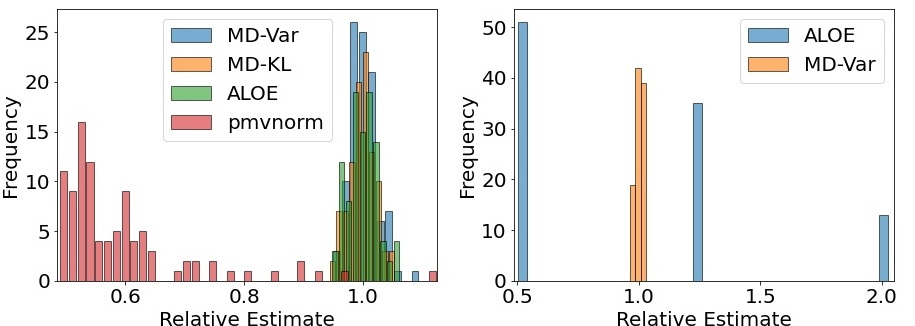
\includegraphics[width=.95\textwidth]{Dissertation/images/sampling/histograms.jpg}
    %\vspace{-.5mm}
    %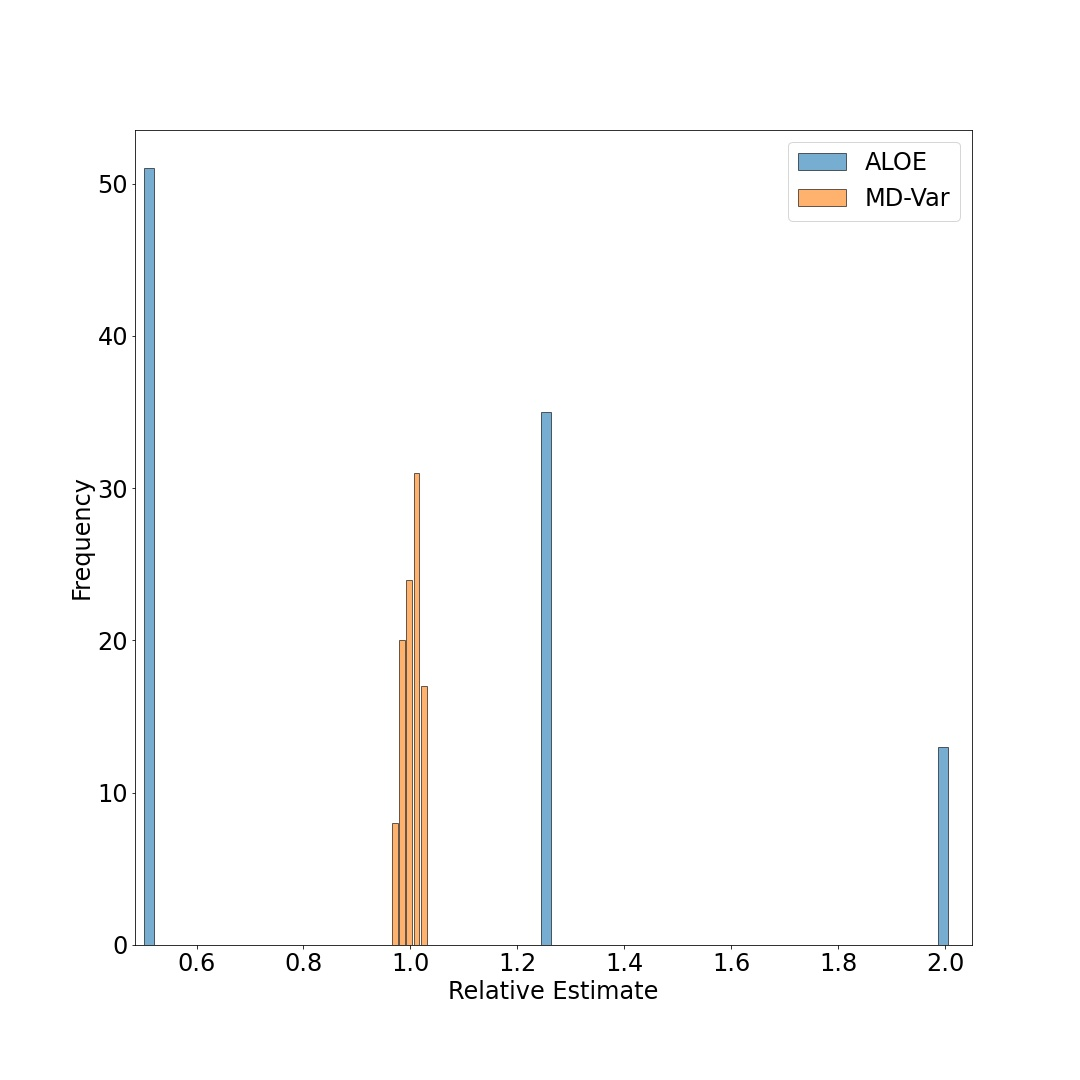
\includegraphics[width=.22\textwidth]{Dissertation/images/sampling/histogram_degenerate.jpg}%\hspace{-3mm}
    %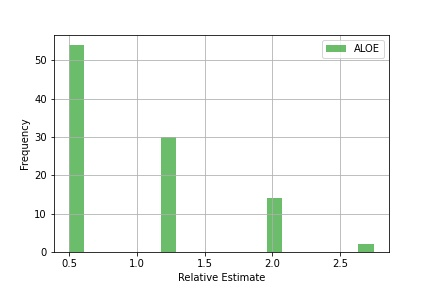
\includegraphics[width=.25\textwidth]{Dissertation/images/sampling/IS_hists_shivering_only_OMC.jpg}
    \caption{Importance 
    sampling methods performance on a 2-dimensional (left) regular polytope with $360$ faces; (right) degenerate polytope with $1500$ faces. Overload probabilities are  $\Phi(-6)$ and $2\Phi(-1)$ resp. 
    }
    \label{fig:01}
    % \vspace{-5mm}
%\end{figure}
%\begin{figure}[t!]
%    \centering
    %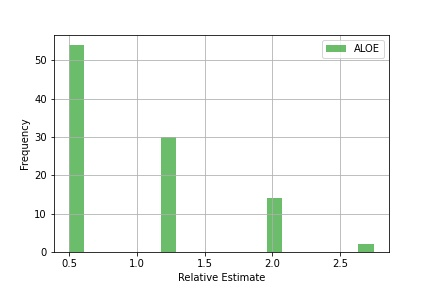
\includegraphics[width=.25\textwidth]{Dissertation/images/sampling/IS_hists_shivering_only_OMC.jpg}
    %\caption{Importance 
    %sampling methods performance on a 2-dimensional degenerate polytope with $1500$ faces and overload probability $2\Phi(-1)$.}
    %\label{fig:degenerate_polytope}
    %\vspace{-5mm}
\end{figure}

%Moreover, we would like to address the question of sampling complexity's dependence on the number of planes and true event probability. See Figure~\ref{fig:complexities}. We declare that the algorithm has converged once the relative difference between two subsequently produced standard deviations of the estimate are small enough: $|\texttt{std}_i - \texttt{std}_{i+1}| / \texttt{std}_{1000} \leq 10^{-3}$. 
%{\color{red} Sasha, please change it as we discuss. The criteria above does not make any sense because of the numerical instability}
%Here we can observe that the smaller probability than it is more samples required to estimate that for MC. ALOE and proposed methods, i.e., Mirror Descent based, seems to be not caring much about the true probability. Also, we observe that the proposed mirror descent based approaches are much more efficient.



\paragraph{Degenerate polytope} Although ALOE is one of the best choices for a regular polytope, the algorithm does not take into account the joint geometry of various hyperplanes. 
%
As the second example we consider a degenerate polytope with $K=1500$ faces, where $\omega_1 = (0, 1)$  and $\omega_k = (\xi, -1 - \xi)$, $2\le k \le K$. We take $\xi \sim \mathcal{U}[-\varepsilon, \varepsilon]$ for small $\varepsilon = 10^{-6}$. Note that $\omega_k$ for $k\geq 2$ are almost identical. Hence probability $\Pi$ is quite close to $2\Phi(-\tau)$. In this experiment, ALOE puts a lot of efforts on sampling points in the area $\{p: (0, -1)^\top p \ge \tau\}$, while the set $\{p: \omega_1^\top p \ge \tau\}$ remains unexplored which leads to a higher variance of the sampler and a less efficient method compared to the proposed optimization approach. Figure~\ref{fig:01} illustrates the performance of ALOE in this case. 

\paragraph{Power Grid Cases} In this subsection we consider real-world polytopes corresponding to DC power grids (IEEE test cases) and Gaussian power injections.
%
%We also compare the algorithms' efficiency in solving the  on various IEEE test cases. s
%by comparing the algorithms' efficiency over various IEEE test cases. 
%
We ran the algorithms on all the test cases  accessible through PandaPower~\cite{pandapower.2018}. There were 27 cases with the number of buses varying from 4 to 9241. The proposed methods (MD-Var and MD-KL) took less than two minutes of computational time on a personal laptop for each of them. 
%
Table~\ref{tab:sample-compX} shows the minimal number of samples that are required by the algorithms to achieve 
\begin{align}
    \Pi/2 \le \hat\Pi \pm s(\hat\Pi) \le 3\Pi/2, \label{eq:tk}
\end{align}
where $s(\hat\Pi)$ is the empirical standard deviation of the estimate. This ensures that not only the estimated value, but also its confidence interval is contained in $(\Pi/2, 3\Pi/2)$ and that the sum of the empirical estimate and its standard deviation are close to %of the same order as 
the true probability. 


\begin{table}[ht]
\centering
%\vspace{-4mm}
% \captionsetup{justification=centering}
\caption{Number of samples to satisfy Ineq.~\eqref{eq:tk} 
 for Iceland118}
 \begin{tabular}{|c|c|c|c|c|} 
 \toprule
 \hspace{-2mm}Bound ${\bar\theta}_{ij}$, probability $\Pi$ & MC & ALOE & Pmvnorm & MD-Var\\
 % &&& \cite{genz2020package} & (Section \ref{sampling:nm})\\
 \hline
  \hspace{-2mm}$|{\theta}_{ij}| \le \pi/8$, $\Pi$ = 1.2e-01 & 6.4e+02 & 3.7e+02 & \underline{3.2e+02} & 4.1e+02\\
  \hspace{-2mm}$|{\theta}_{ij}| \le \pi/7$, $\Pi$ = 3.0e-02 & 5.1e+04 & 4.1e+02 & 1.1e+03 & \underline{3.5e+02}\\
  \hspace{-2mm}$|{\theta}_{ij}| \le \pi/6$, $\Pi$ = 2.5e-03  & 6.2e+06 & 4.5e+02 & 6.3e+03 & \underline{3.9e+02} \\
  \hspace{-2mm}$|{\theta}_{ij}| \le \pi/5$, $\Pi$ = 2.6e-05  & 8.9e+10 & 3.3e+02 & 1.4e+04 & \underline{2.1e+02}\\
  \bottomrule
 \end{tabular}
 \vspace{-3mm}\label{tab:sample-compX}
\end{table}


Table~\ref{tab:emp} shows overload probability estimates and their standard deviations for the algorithms based on $N = 200$ samples on various PandaPower~\cite{pandapower.2018} power grids. In all the presented cases except for the Iceland grid, we set the standard deviations of output powers of generators to $0.25$ of their average values. For the Iceland test case, we use $0.1$ instead of $0.25.$ 
Pmvnorm~\cite{genz2020package} did not terminate on Polish 3120sp case after an hour of computations which we indicated as N/A. All other methods terminate in less than a minute. The proposed algorithms reduce variance and are more computationally efficient than the state-of-the-art ALOE and pmvnorm. Fig.~\ref{fig:weights118}~shows~a~substantial change in hyperplane weight assignment made by MD-Var. Our code is publicly available on Github at \url{https://github.com/vjugor1/adaptive_importance_sampling_power_grids}. 

%how convex optimization 
%% To reviewers' response
%Another field to be considered is the weights in the mixture. Figure~\ref{fig:weights118} shows the distribution of top weights in the $\textit{MD}_{\textit{V}}$ and ALOE's mixtures for the Iceland118 case with fluctuations of $0.1$ magnitude and maximum phase difference of $\pi / 3$. We have not included $\textit{MD}_{\textit{KL}}$ for the sake of clearer presentation, since it yielded almost the same weights as the $\textit{MD}_{\textit{V}}$. We can observe that the optimization approach brings out the most crucial (from the failure point of view) component higher and leaves the rest almost untouched.

% %To further investigate the variance behaviour, let us see Figure~\ref{fig:3120}. 
% %Here we can see that the proposed algorithms dominate the ALOE in terms of variance thought the whole sampling process. $\textit{MD}_{\textit{V}}$, non-surprisingly, has better variance than $\textit{MD}_{\textit{KL}}$, since the former is aimed at variance optimization.

% %\begin{figure}[h]
% %    \centering
% %    \vspace{-3mm}
% %    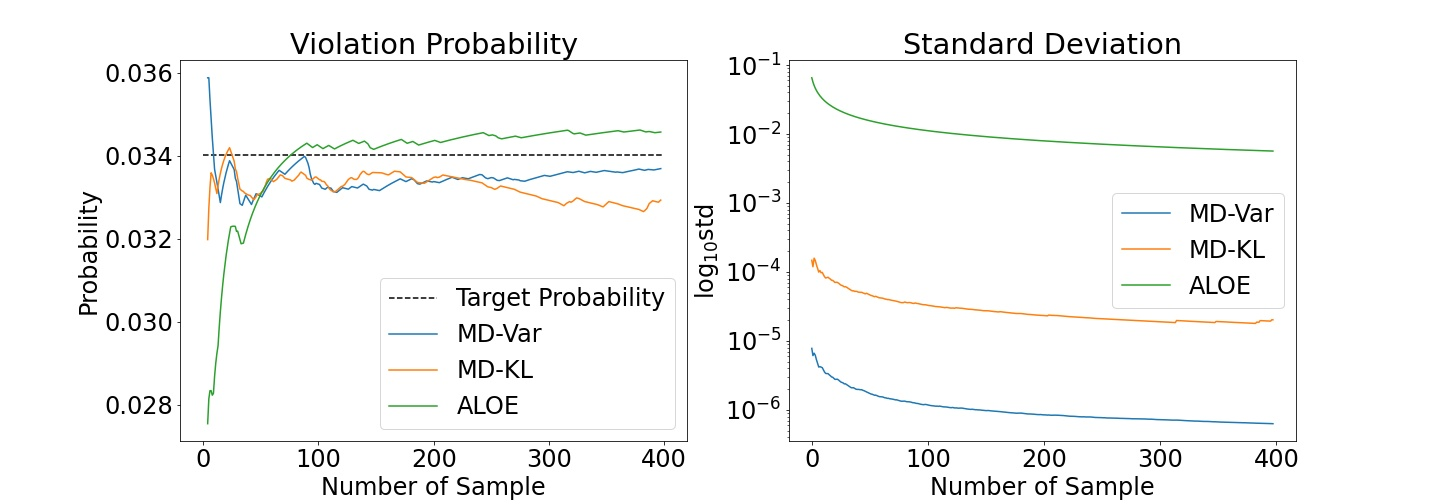
\includegraphics[width=.55\textwidth]{Dissertation/images/sampling/grid3120with_pmv.jpg}
% %    \vspace{-3mm}
% %    \caption{Convergence plots for the probability estimates (left) and standard deviation of the estimates (right) for the Polish3120 grid. Maximum angle difference is $\pi/4$ and the fluctuation are $0.25$ of magnitudes.}
% %    \label{fig:3120}
% %    \vspace{-4mm}
% %\end{figure}


% %Another field to be considered is the weights in the mixture. Figure~\ref{fig:weights118} shows the distribution of top weights in the $\textit{MD}_{\textit{V}}$ and ALOE's mixtures for the Iceland118 case with fluctuations of $0.1$ magnitude and maximum phase difference of $\pi / 3$. We have not included $\textit{MD}_{\textit{KL}}$ for the sake of clearer presentation, since it yielded almost the same weights as the $\textit{MD}_{\textit{V}}$. We can observe that the optimization approach brings out the most crucial (from the failure point of view) component higher and leaves the rest almost untouched.

\begin{figure}[t]
    \centering
    %\vspace{-1mm}
    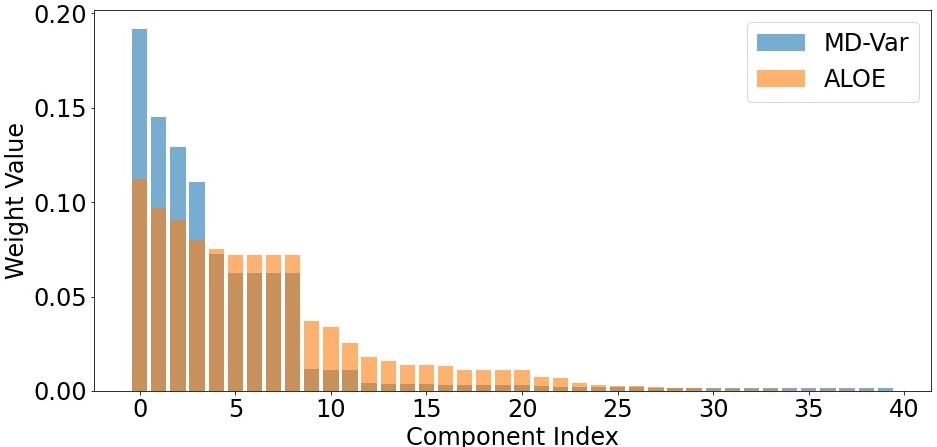
\includegraphics[width=.95\textwidth]{Dissertation/images/sampling/weights_pi3_grid118i.jpg}
    %\vspace{-2mm}
    \captionsetup{justification=centering}
    \caption{Weights of mixture distribution %\eqref{eq:mix} 
    assigned by ALOE and MD-Var for Iceland 118 case with phase angle limit $\pi/3$ and a standard deviation of power injection on generators equal to $0.1$ of its average.}
    \label{fig:weights118}
    % \vspace{-2mm}
\end{figure}



% \begin{comment}
% Finally, as the ground truth we use an estimate of failure given after $N=10000$ iterations of ALOE~\cite{owen2019importance} and set $\Pi$ equal to it in Table~\ref{tab:emp}. We set a deviation on generators (except the slack bus) to be 0.1 of net power injections, i.e. the difference between power generation and consumption. Finally, we set variance on loads equals to zero. \end{comment}




\begin{table}[t]
    \centering
    % \captionsetup{justification=centering}
    \caption{Overload probability estimation for power grids.}
    \label{tab:emp}
    \begin{tabular}{|l|l|l|l|l|l|l|}
    \toprule
          Estimate, $\hat\Pi$ & $\bar\theta$ & $\Pi$ &  \text{ALOE} & MD-Var & MD-KL & pmvnorm\\
          \hline
          \multicolumn{7}{c}{IEEE 30}\\
          \hline
$\hat\Pi \times$ 1e+15 & $\pi/4$\hspace{-4mm}&8.2\!\! & 8.2 $\pm$ 0.9 & 8.2 $\pm$ 0.0 & 8.2 $\pm$  0.0 & 8.2 $\pm$ 1.2 \\
$\hat\Pi \times$ 1e+06 & $\pi/6$\hspace{-4mm}&5.8\!\! & 5.8 $\pm$ 0.7 & 5.8 $\pm$ 0.0 & 5.8 $\pm$ 0.0 & 5.8 $\pm$ 1.0 \\
$\hat\Pi \times$ 1e+04 & $\pi/7$\hspace{-4mm}&2.9\!\! & 2.9 $\pm$ 0.3 & 2.9 $\pm$ 0.0 & 2.9 $\pm$ 0.0 & 2.9 $\pm$ 0.5\\
$\hat\Pi \times$ 1e+03 & $\pi/8$\hspace{-4mm}&3.1\!\! & 3.1 $\pm$ 0.4 & 3.1 $\pm$ 0.0 & 3.1 $\pm$ 0.1 & 3.1 $\pm$ 0.4\\
\hline
\multicolumn{7}{c}{IEEE 57}\\
\hline
$\hat\Pi \times$ 1e+03 & $\pi/2$\hspace{-4mm}&8.8\!\! & 9.1 $\pm$ 0.8 & 8.7 $\pm$ 0.0 & 8.8 $\pm$ 0.0 & 8.9 $\pm$ 1.2\\
$\hat\Pi \times$ 1e+02 & $\pi/3$\hspace{-4mm}&8.4\!\! & 8.5 $\pm$ 1.1 & 8.4 $\pm$ 0.1 & 8.3 $\pm$ 0.5 & 9.0 $\pm$ 0.9\\
%$\hat\Pi \times$ 1e+01 & $\pi/4$\hspace{-4mm}&2.0\!\! & 2.0 $\pm$ 0.2 & 2.0 $\pm$ 0.0 & 1.9 $\pm$ 0.7 & 2.0 $\pm$ 0.0\\
%$\hat\Pi \times$ 1e+01 & $\pi/6$\hspace{-4mm}&4.1\!\! & 4.1 $\pm$ 0.3 & 4.2 $\pm$ 0.5 & 4.3 $\pm$ 1.0 & 4.1 $\pm$ 0.0\\
          \hline
          \multicolumn{7}{c}{Iceland 118}\\
          \hline
$\hat\Pi \times$ 1e+09 & $\pi/2$\hspace{-4mm}&6.2\!\! & 6.2 $\pm$ 0.1 & 6.1 $\pm$ 0.0 & 6.1 $\pm$ 0.0 & 5.7 $\pm$ 2.6\\
$\hat\Pi \times$ 1e+04 & $\pi/3$\hspace{-4mm}&2.8\!\! & 3.0 $\pm$0.0 & 2.9 $\pm$ 0.0 & 2.9 $\pm$ 0.0 & 2.8 $\pm$ 1.4\\
$\hat\Pi \times$ 1e+02 & $\pi/4$\hspace{-4mm}&1.1\!\! & 1.1 $\pm$ 0.2 & 1.1 $\pm$ 0.0 & 1.1 $\pm$ 0.0 & 1.1 $\pm$ 0.2\\
$\hat\Pi \times$ 1e+01 & $\pi/6$\hspace{-4mm}&1.4\!\! & 1.4 $\pm$ 0.2 & 1.4 $\pm$ 0.0 & 1.3 $\pm$ 0.0 & 1.4 $\pm$ 0.1\\
\hline 
          \multicolumn{7}{c}{Illinois 200}\\
\hline
$\hat\Pi\times$ 1e+12 & $\pi/4$\hspace{-4mm}&7.9\!\! & 7.9 $\pm$ 0.9 & 7.9 $\pm$ 0.0 & 7.9 $\pm$ 0.0 & 7.9 $\pm$ 3.3\\
$\hat\Pi\times$ 1e+04 & $\pi/6$\hspace{-4mm}&1.1\!\! & 1.1 $\pm$ 0.1 & 1.1 $\pm$ 0.0 & 1.1 $\pm$ 0.0 & 1.1 $\pm$ 0.3\\
$\hat\Pi\times$ 1e+03 & $\pi/7$\hspace{-4mm}&2.3\!\! & 2.3 $\pm$ 0.2 & 2.3 $\pm$ 0.0 & 2.3 $\pm$ 0.0 & 2.3 $\pm$ 0.3\\
$\hat\Pi\times$ 1e+02 & $\pi/8$\hspace{-4mm}&1.5\!\! & 1.5 $\pm$ 0.1 & 1.5 $\pm$ 0.0 & 1.5 $\pm$ 0.0 & 1.5 $\pm$ 0.1\\
\hline
\multicolumn{7}{c}{Polish 3120sp}\\
\hline
$\hat\Pi\times$ 1e+13 & $\pi/2$\hspace{-4mm}&3.7\!\! & 3.7 $\pm$ 0.4 & 3.7 $\pm$ 0.0 & 3.7 $\pm$ 0.0 & N/A\\
$\hat\Pi\times$ 1e+04 & $\pi/3$\hspace{-4mm}&1.2\!\! & 1.2 $\pm$ 0.1 & 1.2 $\pm$ 0.0 & 1.2 $\pm$ 0.0 & N/A\\
$\hat\Pi\times$ 1e+02 & $\pi/4$\hspace{-4mm}&3.4\!\! & 3.4 $\pm$ 0.5 & 3.4 $\pm$ 0.3 & 3.4 $\pm$ 0.6 & N/A\\
\bottomrule
    \end{tabular}
    %\vspace{-4mm}
\end{table}




\section{Conclusion}\label{sampling:conclusion}

Importance sampling is a useful tool for real-time reliability assessment in power grids. We proposed an algorithm that, first, constructs a physics-informed mixture distribution for importance sampling, and, second, utilizes convex optimization to adjust the weights of the mixture.  The method outperforms state-of-the-art algorithms in accuracy and efficiency of reliability assessment. We hope that this approach can be further used for optimization and control in power grids. %importance sampling can ... used for control purposes

% % \bibliographystyle{IEEEtran}
% % \bibliography{biblio}
